\section{Introduction}

Effective bankroll management is a critical component of successful sports betting. It involves determining the optimal amount to wager on each bet to maximize growth while minimizing the risk of ruin. This section details the development and evaluation of an optimization module designed to calculate the optimal fraction of the bankroll to invest in each betting opportunity. The module leverages probabilistic forecasts from the predictive models discussed in the previous section and applies various investment strategies, including the Kelly criterion, expected value maximization, and naive betting approaches.

\section{Methodology}
\subsection{Investment Strategies}

This section provides an overview of the different bankroll allocation strategies implemented, ranging from naive methods to more advanced optimization techniques. The focus is on the principles guiding each strategy, with a detailed formula provided only for the naive strategy.

\subsubsection{List of Strategies}

\begin{itemize}
    \item \textbf{Kelly Criterion Strategy}: \cite{Kelly1956} \cite{Thorp1969}  
    This strategy maximizes the logarithmic utility of wealth, aiming for long-term bankroll growth while managing risk. The bankroll fractions are derived from the analytical solution using the approximations  \ref{appendix:analytical_solution_using_the_kelly_criterion}, \(\mathbb{E}(U(B)) = \mathbb{E}(B) - \frac{1}{2} \cdot \mathbb{V}\text{ar}(B) \) which comes down to a Linear utility strategy using \( \lambda = \frac{1}{2} \).

    \item \textbf{Log Utility Strategy}:  
    Similar to the Kelly criterion, this strategy focuses on maximizing the expected logarithmic utility \(U(B) = \ln(B)\)  but using no approximations \ref{appendix:analytical_reduction_using_log_expected_utility}.

    \item \textbf{Exponential Utility Strategy}:  
    This strategy uses an exponential utility function \(U(B) = -e^{-\alpha B}\) to take into account the bettor’s risk aversion, balancing between expected returns and risk tolerance \ref{appendix:analytical_reduction_using_exp_expected_utility}.

    \item \textbf{Linear Utility Strategy}:
    In this strategy, the objective is to maximize the trade-off between expected returns and risk, represented by the function \(\mathbb{E}(U(B)) = \mathbb{E}(B) - \lambda \cdot \mathbb{V}\text{ar}(B) \). For the simulations, we set \( \lambda = 10 \), reflecting a high level of risk aversion. This approach seeks to maximize returns while penalizing high variance, aiming to balance growth and stability \ref{appendix:analytical_solution_using_linear_expected_utility}. 

    \item \textbf{Expected Value Maximization Strategy}:  
    This strategy optimizes bankroll allocation based purely on maximizing expected value, \(U(B) = B\), without considering risk or variance.

    \item \textbf{Naïve Strategy: Bet on the Most Likely Outcome}:  
    In this straightforward approach, the bettor places the entire bet on the outcome with the highest implied probability, as per the bookmaker's odds.
    
    The formula for this strategy is:
    \[
    f_{k,i} = 
    \begin{cases}
    \frac{1}{M}, & \text{if } i = \arg\max(o_k) \\
    0, & \text{otherwise}
    \end{cases}
    \]
    where:
    \begin{itemize}
        \item \( f_{k,i} \) is the fraction of the bankroll wagered on outcome \( i \) of match \( k \),
        \item \( o_k \) are the odds for match \( k \).
        \item \(M\) is the number of matches available.
    \end{itemize}
    This strategy is simple and allocates all the available funds to the outcome with the highest bookmaker odds.
\end{itemize}

These strategies were benchmarked against each other in the Monte Carlo simulations and then Online testing to assess their effectiveness in managing risk and maximizing bankroll growth. \\

For each strategy, a factor of \( \gamma = \frac{1}{2} \) was applied to the bet fractions to ensure that not the entire bankroll was wagered at any given time, thereby providing a margin of safety, such as: \(f_{strategy\_final} = \gamma \times f_{strategy}\).


\subsection{Optimization Algorithms}

Two optimization algorithms were employed to solve the bankroll allocation problem \cite{BoydVandenberghe2004}:

\begin{itemize}
    \item \textbf{Sequential Least Squares Programming (SLSQP):} An iterative method for constrained nonlinear optimization that is efficient for problems with a moderate number of variables.
    \item \textbf{Trust-Region Constrained Algorithm (trust-constr):} Suitable for large-scale optimization problems, it handles large numbers of variables and constraints effectively.
\end{itemize}

The choice between SLSQP and trust-constr depends on the number of betting opportunities (matches) considered at once. For a large number of matches, trust-constr is preferred due to its scalability.


\section{Monte Carlo Simulations}

To assess the performance of different investment strategies under simulated sports betting conditions, we conducted Monte Carlo simulations modeling the inherent uncertainties. The goal was to evaluate how various bankroll allocation strategies perform over numerous trials.

\subsection{Simulation Setup}

We simulated true match outcome probabilities \( r \) using a Dirichlet distribution appropriate for mutually exclusive and collectively exhaustive events:

\[
r_i^k = \text{Dirichlet}(\alpha), \quad \alpha = (1, 1, 1)
\]

To introduce discrepancies between true probabilities and those estimated by bookmakers (\( b \)) and players (\( t \)), we added biases and normally distributed noise:

\[
b_i^k = \text{clip}(r_i^k + \text{bias}_{\text{bookmaker}} + \epsilon_{\text{bookmaker}}, \ \text{min\_prob}, \ \text{max\_prob})
\]
\[
t_i^k = \text{clip}(r_i^k + \text{bias}_{\text{player}} + \epsilon_{\text{player}}, \ \text{min\_prob}, \ \text{max\_prob})
\]

where \( \epsilon_{\text{bookmaker}}, \epsilon_{\text{player}} \sim \mathcal{N}(0, \sigma^2) \). Probabilities were normalized to sum to one, and bookmaker probabilities included a margin \( \text{margin}_{\text{bookmaker}} \), clipping between \text{min\_prob} and \text{max\_prob}. Bookmaker odds were calculated as:

\[
o_i^k = \frac{b_i^k}{(\sum_{i=0}^N b_i^k) - \text{margin}_{\text{bookmaker}}}
\]

\subsection{Simulation Procedure}

The simulation followed a structured approach to evaluate the performance of different betting strategies, using predefined constants and a series of steps to simulate match outcomes and bankroll updates.

\begin{table}[H]
\centering
\caption{Simulation constants}
\label{tab:simulation constants}
\begin{minipage}{.2\linewidth}
\centering
\begin{tabular}{lr}
\toprule
\textbf{Constant} & \textbf{Value}\\
\midrule
H & 30 \\
T & 50 \\
N & 3 \\
\(\text{min\_prob}\) & 0.05 \\
\(\text{max\_prob}\) & 0.95 \\
\bottomrule
\end{tabular}
\end{minipage}%
\hspace{0.05\linewidth}
\begin{minipage}{.45\linewidth}
\centering
\begin{tabular}{lrr}
\toprule
\textbf{Constant} & \textbf{Bettor} & \textbf{Bookmaker}\\
\midrule
\text{bias} & 0 & 0 \\
\(\sigma\) (for noise \(\epsilon)\) & 0.1 & 0.1 \\
\text{margin} &  & 0.1 \\
\bottomrule
\end{tabular}
\end{minipage}
\end{table}

\begin{enumerate}
    \item Generated true probabilities \( r \) using \(\text{bias} = 0\) and \(\epsilon = 0.1\) for both bettor and bookmaker.
    \item Computed bookmaker and player estimates \( b \) and \( t \).
    \item Calculated bookmaker odds \( o \).
    \item For each strategy:
    \begin{itemize}
        \item Determined bet sizes using \( t \) and \( o \) by performing optimisation using \texttt{truct\_constr} algorithm.
        \item Simulated match outcomes based on \( r \).
        \item Updated bankrolls accordingly.
    \end{itemize}
\end{enumerate}

\subsection{Evaluation Metrics}

Strategies were evaluated using:

\begin{itemize}
    \item \textbf{Final Bankroll Statistics}: Mean, standard deviation, median, minimum, and maximum.
    \item \textbf{Average Growth Rate}: Geometric mean per time step. 
    \[GGR = \left( \frac{B(n)}{B(0)} \right)^{\frac{1}{n}} - 1\]

    \item \textbf{Sharpe Ratio}: Risk-adjusted return.

    \[\text{Sharpe Ratio} = \frac{\frac{1}{n} \sum_{t=1}^{n} R(t)}{\mathbb{V}ar(R(t))}) \text{   with   } R(t) = \frac{B(t+1) - B(t)}{B(t)}\]
    
    \item \textbf{Probability of Ruin}: Frequency of bankroll falling below a threshold.
\end{itemize}

\subsection{Results}

\begin{figure}[H]
    \centering
    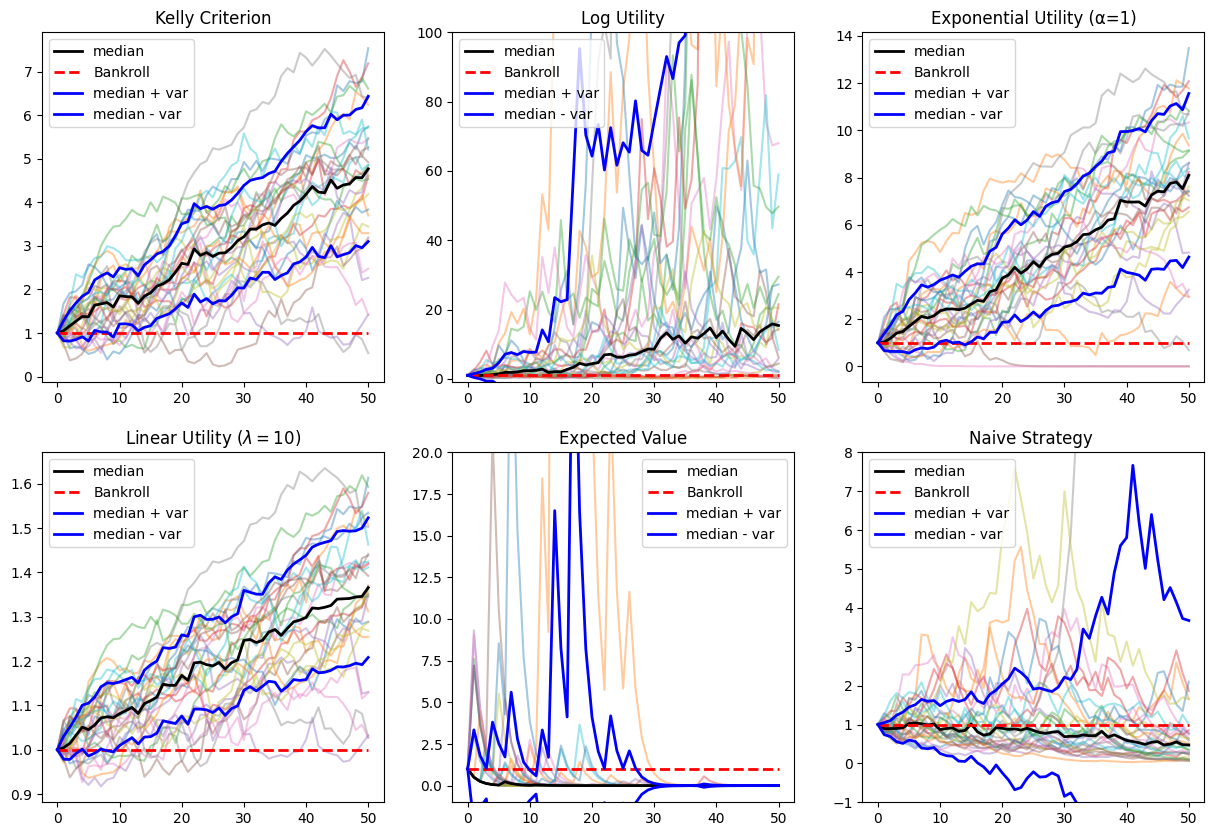
\includegraphics[width=1.1\textwidth, keepaspectratio]{images/monte_carlo_b=b.png}
    \caption{Monte carlo simulations for each strategy}
    \label{fig:monte_carlo}
\end{figure}


\begin{table}[H]
\centering
\caption{Final Bankroll Statistics}
\label{tab:final_bankroll}
\begin{tabular}{lrrrrr}
\toprule
\textbf{Strategy} & \textbf{Mean} & \textbf{Std Dev} & \textbf{Median} & \textbf{Min} & \textbf{Max} \\
\midrule
Kelly Criterion          & 4.48   & 1.67   & 4.77   & 0.54   & 7.54   \\
Log Utility              & 270.85 & 983.14 & 15.39  & 0.19   & 5414.01 \\
Exponential Utility      & 7.46   & 3.46   & 8.10   & 0.00   & 13.48  \\
Linear Utility           & 1.35   & 0.16   & 1.37   & 1.03   & 1.61   \\
Expected Value           & 0.00   & 0.00   & 0.00   & 0.00   & 0.01   \\
Naïve Strategy           & 1.20   & 3.20   & 0.47   & 0.06   & 18.19  \\
\bottomrule
\end{tabular}
\end{table}

The \textbf{Log Utility} strategy achieved the highest mean final bankroll but with significant variability, indicating high risk. The \textbf{Kelly Criterion} and \textbf{Exponential Utility} strategies demonstrated moderate returns with lower variability, suggesting consistent performance.

\begin{table}[H]
\centering
\caption{Average Growth Rate Per Step}
\label{tab:avg_growth}
\begin{tabular}{lr}
\toprule
\textbf{Strategy} & \textbf{Growth Rate} \\
\midrule
Kelly Criterion          & 2.82\% \\
Log Utility              & 5.54\% \\
Exponential Utility      & 2.55\% \\
Linear Utility           & 0.59\% \\
Expected Value           & $-$29.83\% \\
Naïve Strategy           & $-$1.55\% \\
\bottomrule
\end{tabular}
\end{table}

While the \textbf{Log Utility} strategy had the highest growth rate, it came with increased volatility. The \textbf{Kelly Criterion} and \textbf{Exponential Utility} strategies offered positive growth with better risk control.

\begin{table}[H]
\centering
\caption{Sharpe Ratio}
\label{tab:sharpe_ratio}
\begin{tabular}{lr}
\toprule
\textbf{Strategy} & \textbf{Sharpe Ratio} \\
\midrule
Kelly Criterion          & 0.30 \\
Log Utility              & 0.29 \\
Exponential Utility      & 0.25 \\
Linear Utility           & 0.30 \\
Expected Value           & 0.14 \\
Naïve Strategy           & 0.01 \\
\bottomrule
\end{tabular}
\end{table}

The highest Sharpe Ratios were achieved by the \textbf{Kelly Criterion} and \textbf{Linear Utility} strategies, indicating superior risk-adjusted returns.

\begin{table}[H]
\centering
\caption{Probability of Ruin}
\label{tab:prob_ruin}
\begin{tabular}{lr}
\toprule
\textbf{Strategy} & \textbf{Probability} \\
\midrule
Kelly Criterion          & 0.00\% \\
Log Utility              & 3.33\% \\
Exponential Utility      & 6.67\% \\
Linear Utility           & 0.00\% \\
Expected Value           & 100.00\% \\
Naïve Strategy           & 20.00\% \\
\bottomrule
\end{tabular}
\end{table}

Zero probability of ruin for the \textbf{Kelly Criterion} and \textbf{Linear Utility} strategies underscores their robustness.

An ANOVA test (performed to assess whether the differences in final bankrolls among the strategies), (F-statistic: 2.16, p-value: 0.0612) suggested that differences among strategies were not statistically significant at the 5\% level. However, the p-value is close to the threshold, suggesting that with a larger sample size, the differences might become statistically significant.

\subsection{Conclusion}

The simulations indicate that strategies like the \textbf{Kelly Criterion} and \textbf{Exponential Utility}, which balance growth and risk through utility maximization, offer favorable outcomes. The \textbf{Log Utility} strategy provides high growth potential but with greater volatility. Ignoring risk, as in the \textbf{Expected Value} strategy, leads to poor performance.

\textbf{Limitations} include the limited number of simulations, simplified assumptions, and exclusion of real-world factors like transaction costs.

\textbf{Recommendations} for future work involve increasing simulation runs, incorporating realistic market conditions, and exploring additional strategies.


\section{Online Testing}

To assess the strategies in a real-world environment, an online testing phase was conducted over five weeks, from 2024 August 24th to 2024 September 30th, focusing on matches from the five major European football leagues. This real-world testing evaluated the practical applicability and performance of the strategies under actual market conditions. Odds were scraped each day at 12pm from the Odd Api website.


\subsection{Static Problem Reduction and Parameter Settings}

To simplify the dynamic nature of sports betting, we reduced the problem to a series of static optimizations at discrete time intervals. At each decision point \( t \), bankroll allocation was optimized based on the current available information. This approach allowed us to manage the complexity of real-time betting while ensuring the practical applicability of the strategies.

\paragraph{Temporal Parameters}

Key temporal parameters were defined as follows:

\begin{itemize}
    \item \textbf{Betting Interval (\( \Delta t \))}: The interval between placing bets, set to 24 hours to capture daily betting opportunities.
    \item \textbf{Bet Placement Timing}: Bets were placed at a fixed time each day (12:00 PM) to ensure up-to-date information was used while accommodating market dynamics.
\end{itemize}

These settings ensured a balance between information accuracy and practical market conditions.

\paragraph{Match Selection}

The matches selected for each optimization were determined based on:

\begin{itemize}
    \item \textbf{Number of Matches (\( M \))}: Matches occurring within the next 24 hours were selected, balancing opportunity and reliability of information as well as having all results while perfomring next step.
    \item \textbf{Selection Criteria}: Focus was given to matches from top European leagues where the bettor had a higher perceived edge.
\end{itemize}

This careful match selection helped reduce computational complexity while enhancing potential returns.

\paragraph{Re-Betting Policy}

The re-betting policy was defined by the following criteria:

\begin{itemize}
    \item \textbf{Not allowing Re-Bets}: Additional bets on previously considered matches were not allowed. As we only bet on matches on the same day and only once a day, this was an implication of the previous choices.
\end{itemize}

This policy helped manage risk and adapt to evolving market conditions.

\subsection{Practical Implementation Settings}

The practical implementation settings for the online testing phase are summarized in Table~\ref{tab:implementation_settings}. The testing period ran from August 24, 2024, to September 30, 2024. The \texttt{trust-constr} algorithm was used for optimization, with a multiplier of \( \gamma = \frac{1}{2} \) applied to the matrix \( f \). The best odds from a pool of bookmakers (detailed in the appendix) were selected for each match.

\begin{table}[H]
\centering
\caption{Practical Implementation Settings}
\label{tab:implementation_settings}
\begin{tabular}{ll}
\toprule
\textbf{Setting}               & \textbf{Value}                                 \\ \midrule
Betting Interval (\( \Delta t \))     & 24 hours \\                                    
Bet Placement Time               & 12:00 PM daily                                \\
Look-Ahead Horizon               & Matches within the next 24 hours               \\ 
Re-Betting Policy                & Not allowed \\ 
Testing Period                   & August 24, 2024 – September 30, 2024           \\ 
Optimization Algorithm           & \texttt{trust-constr}                          \\ 
Strategy factor mult. \(\gamma\)         & \( 0.5 \)                              \\ 
Odds Selection                   & Biggest odds from a pool of bookmakers            \\ 
Markets & 5 biggest European leagues (Big 5) \\
\bottomrule
\end{tabular}
\end{table}


\subsection{Results and Interpretation}

Figure~\ref{fig:capital_evolution} illustrates the capital evolution for each strategy during the testing period. The Kelly and Exponential Utility strategies exhibited the strongest performance, both ending with approximately twice the initial capital. These results highlight their ability to optimally balance risk and reward, consistently outperforming the more conservative Log and Naive strategies. However, they also demonstrated higher volatility compared to the more stable Linear strategy.

\begin{figure}[H]
    \centering
    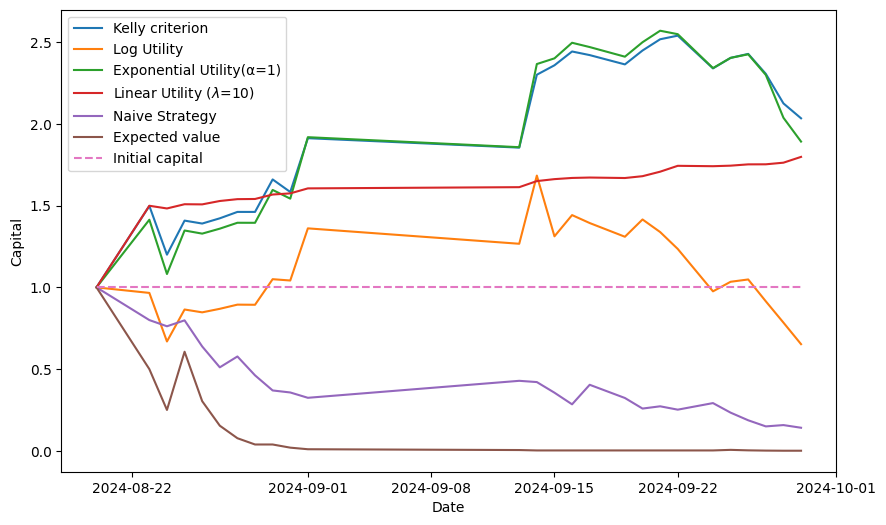
\includegraphics[width=\textwidth]{images/bankroll_evolution2.png}
    \caption{Capital Evolution for Each Strategy During the Online Testing Period}
    \label{fig:capital_evolution}
\end{figure}

The Log Utility strategy underperformed, particularly at the start and after the midpoint of the test period, failing to capitalize on high-return opportunities. Its conservative nature, aimed at minimizing risk, resulted in modest growth but ultimately led to a negative outcome. 

Both the Naive and Expected Value strategies experienced sharp declines in capital. The Naive strategy approached near-zero capital by the end of the test, while the Expected Value strategy exhibited extreme volatility, leading to rapid capital depletion. These simpler strategies, which lack sophisticated optimization, were highly vulnerable to adverse market conditions and failed to adapt effectively to fluctuations in odds or match outcomes.

In contrast, the Linear Utility strategy showed steady and consistent growth, with minimal volatility throughout the testing period, ultimately achieving a final growth of 1.8 times the initial capital. This highlights its effectiveness in maintaining a stable growth trajectory while avoiding the excessive risk associated with other strategies.

Overall, the results underscore the superiority of more advanced utility-based strategies such as Kelly and Linear. These approaches consistently outperformed simpler methods by balancing risk and reward more effectively under real-world betting conditions.

\subsection{Performance Metrics}

To further quantify the performance of each strategy, we computed key metrics, including final bankroll \( B(T) \), mean growth per step, and standard deviation of growth per step, both in absolute terms and as a percentage of the final bankroll. 
\begin{itemize}
    \item The mean growth per step is defined as:
    \[
    \mu = \frac{1}{T-1} \sum_{t=1}^{T-1} \Delta B_t
    \]
    where \( \Delta B_t = B_{t+1} - B_t \),
    \item the standard deviation of growth per step is given by:
    \[
    \sigma = \sqrt{\frac{1}{T-1} \sum_{t=1}^{T-1} (\Delta B_t - \mu)^2}
    \]
\end{itemize}


Table~\ref{tab:strategy_performance} summarizes the results for each strategy.

\begin{table}[H]
\centering
\caption{Strategy Performance Metrics}
\label{tab:strategy_performance}
\begin{tabular}{llll}
\toprule
\textbf{Strategy}              & \textbf{Final Bankroll \( B(T) \)} & \textbf{Mean Growth (\%)} & \textbf{Std Growth (\%)} \\ 
\midrule
Kelly Criterion                & 2.034                              & 2.034                      & 8.923                    \\ 
Log Utility                    & 0.653                              & -2.129                     & 26.516                   \\ 
Exponential Utility (\( \alpha = 1 \)) & 1.892                        & 1.886                      & 10.309                   \\ 
Linear Utility (\( \lambda = 10 \))    & 1.798                        & 1.776                      & 5.360                    \\ 
Naive Strategy                 & 0.141                              & -24.299                    & 52.419                   \\ 
Expected Value                 & 0.001                              & -5032.448                  & 18175.649                \\
\bottomrule
\end{tabular}
\end{table}

\subsection{Interpretation of Metrics}

The results demonstrate the effectiveness of the Kelly Criterion and Exponential Utility strategies, both of which ended with a final bankroll close to 2.0. These strategies also displayed reasonable volatility, with standard deviations of growth per step under 10\%. The Linear Utility strategy performed consistently, achieving steady growth with the lowest volatility among all strategies.

On the other hand, the Log Utility strategy suffered from negative growth, highlighting its inability to capitalize on high-return opportunities. The Naive and Expected Value strategies performed poorly, with significant capital depletion and extreme volatility, particularly for the Expected Value approach, indicating their inadequacy in real-world betting scenarios.


\section{Conclusion}

The results from both the Monte Carlo simulations and the real-world online testing phase demonstrate the clear advantages of sophisticated bankroll management strategies such as the Kelly Criterion and Exponential Utility methods. These strategies consistently provided strong returns while managing risk effectively, leading to a final bankroll close to twice the initial amount. In contrast, simpler strategies like the Naive and Expected Value approaches underperformed, suffering from capital depletion and high volatility, emphasizing the importance of balancing risk and return in real-world betting scenarios.

The Linear Utility strategy offered a steady, reliable growth trajectory with minimal volatility, making it an appealing option for risk-averse bettors. The Log Utility strategy, though conservative, failed to capture sufficient growth opportunities, resulting in a negative final outcome. Overall, the Kelly and Exponential Utility strategies are best suited for bettors seeking long-term growth with manageable risk.

\subsection{Limitations and Future Improvements}

Despite the promising results, several limitations were identified in the current approach:

\begin{itemize}
    \item \textbf{Simulation Assumptions}: The Monte Carlo simulations relied on several simplifying assumptions that limit the realism of the results. Firstly, the simulation of probabilities was based on the true clipped probabilities plus a bias and Gaussian noise, which does not fully capture the actual flaws in the predictive models, and the constants used were chosen arbitrarily without strong justification. Secondly, the bookmaker margin was fixed, and the odds provided by the bookmaker did not account for the influence of large bets from the players, which in reality could cause deviations in the bookmaker’s odds and probabilities. Lastly, the simulations used a fixed number of matches and time steps. Both the number of simulations and the range of strategies could be expanded to provide a more thorough and diverse analysis of performance over a wider variety of scenarios.
    \item \textbf{Limited Testing Period}: The online testing phase covered only a five-week period, which may not fully capture the long-term performance and robustness of each strategy. Extending the testing period or repeating it across multiple seasons would provide a more comprehensive assessment.
    \item \textbf{Risk Preferences}: While the utility-based strategies successfully managed risk, the models relied on fixed parameters for risk aversion (e.g., \( \lambda \) in Linear Utility). Introducing dynamic adjustments to these parameters based on market conditions or bettor preferences could further enhance performance.
\end{itemize}

\subsection{Future Work and Deployment on Azure Kubernetes}

The next stage of this project involves deploying the entire system on a cloud infrastructure using Kubernetes on Azure (AKS). This deployment will enable scalable, real-time processing of betting opportunities, continuous model updates, and the handling of multiple simultaneous users and markets. By leveraging Azure’s powerful compute and orchestration capabilities, the system will be capable of efficiently managing the computational load and data flows needed for real-time sports betting optimization.

